\section{Experiments}
\label{sec:Evaluation}

\subsection{Setup}
\label{sec:eval-setting}

\textbf{Training details.}
We evaluate representative open-source models across model families and scales: Qwen2.5-\{7B,14B\}~\citep{Yang2024Qwen25TR} on SimpleRL-8k-hard, and Llama3.1-8B~\citep{grattafiori2024llama} on SimpleRL-8k-medium, following the math-domain RLVR recipe~\citep{zeng2025simplerl}.
We evaluate acceleration of RL with GRPO~\citep{shao2024deepseekmath}, using train batch size 128, group size 8, rollout temperature 1.0, and maximum response length 8k for 100 training steps.
All experiments are conducted on a single node with 8 A100-80GB GPUs using data parallelism~\citep{shao2025beat}.

\textbf{System configuration.}
To ensure both deployability and measured speedup, we implement the weight-quantized drafter on top of veRL~\citep{sheng2025hybridflow} and vLLM~\citep{kwon2023efficient}.
Our integration uses the Marlin weight-only quantization kernel~\citep{frantar2025marlin}, which reduces weight-loading cost while preserving compatibility with production-level inference optimizations.
We use a fixed safety margin $\epsilon=0.05$ for \togglepolicy{} and a shared draft-length set $\Gamma=\{5,7,9,11\}$ for \adaptivepolicy{} across all models. Full details are provided in~\cref{app:training_method_config}.

\textbf{Baselines.}
We compare \methodtitle{} against four baselines.
First, \textbf{\nosd{}} denotes accelerated AR inference using the standard rollout backend built on veRL and vLLM~\citep{sheng2025hybridflow,kwon2023efficient}, without SD.
Second, the \textbf{\history{}} baseline evaluates Spec-RL~\citep{liu2025spec}, a rollout-history-based SD method using prefix matching, in the same rollout stack.
We use its best-performing lenience factor $e^{0.5}$, which is needed for meaningful speedup but makes the method lossy and deviate from the target distribution.
Third, the \textbf{\learned{}} baseline evaluates an EAGLE3~\citep{li2025eagle}-based auxiliary drafter implemented on top of veRL and vLLM, following the RL-SD pipelines of FastRL~\citep{hu2026taming} and NeMo RL~\citep{iso2026accelerating}.
We use a fixed draft length of $\DraftLength=3$, following the best-performing setting in~\citet{iso2026accelerating}.
Lastly, \textbf{\alwayssd{}} applies SD with the weight-quantized drafter from~\cref{sec:method}, with SD always enabled.
It uses the same production-level kernel optimization as \methodtitle{}, and we select the best fixed draft length $\DraftLength^{*} \in \{3,5,7\}$ for each configuration.
Additional details on the \history{} and \learned{} baselines are provided in~\cref{app:history_drafting,app:learned_auxiliary_drafting}.

\textbf{Metrics.}
We report per-step averaged latency metrics that separate SD-specific overhead, rollout latency, and end-to-end training time.
Preparation time (Prep.) measures the extra work required by each SD method, including rollout-history lookup, online drafter forward/backward passes and parameter updates, and per-step drafter quantization.
Rollout Gen. measures rollout-generation time, while Step Time measures end-to-end training-step time, including non-rollout components such as log-probability computation and actor updates.
$\mal$, $\bar{\gamma}$, and $\alpha$ denote the average block efficiency, average draft length, and per-token acceptance rate used to compare methods with different $\bar{\gamma}$ values, respectively.
Additional measurement details are provided in~\cref{app:metric_measurement}.

\begin{table*}[t]
\centering
\footnotesize
\setlength{\tabcolsep}{3.6pt}
\renewcommand{\arraystretch}{1.08}
\caption{
End-to-end training acceleration across models and rollout decoding methods.
We report SD-specific preparation time, average block efficiency $\mal$ ($\bar{\gamma}$ denotes the average draft length), per-token acceptance rate $\alpha$, rollout-generation time, and training-step time.
Signed percentages denote relative changes from the \nosd{} baseline.
In arrow-marked columns, bold and underlined entries indicate the \textbf{best} and \underline{second-best} values within each model group.
}
\label{tab:e2e_speedup}
\begin{tabular}{llccccc}
\toprule
\textbf{Model}
&
\textbf{Drafting Method}
&
\textbf{Prep. (s) $\downarrow$}
&
\textbf{$\mal$ / $\bar{\gamma}$}
&
\textbf{$\alpha$ (\%) $\uparrow$}
&
\textbf{Rollout Gen. (s) $\downarrow$}
&
\textbf{Step Time (s) $\downarrow$} \\
\midrule

\multirow{5}{*}{Qwen2.5-7B}
& \nosd{}
& --
& --
& --
& 82.4
& 132.6 \\
& History-based$^\dagger$
& \textbf{1.1}
& N/A
& N/A
& 86.5 (+4.9\%)
& 133.8 (+0.9\%) \\
& Learned auxiliary
& 2.2
& 2.1 / 3.0
& 57.3
& 81.9 (-0.6\%)
& 132.1 (-0.4\%) \\
& \Alwayssd{}
& \underline{1.3}
& 7.5 / 7.0
& \textbf{98.2}
& \underline{75.6 (-8.2\%)}
& \underline{127.6 (-3.7\%)} \\
\rowcolor{gray!10}
\cellcolor{white}
& \methodtitle{}
& \underline{1.3}
& 8.6 / 8.2
& \textbf{98.2}
& \textbf{66.3 (-19.6\%)}
& \textbf{115.7 (-12.7\%)} \\

\midrule

\multirow{5}{*}{Qwen2.5-14B}
& \nosd{}
& --
& --
& --
& 126.6
& 221.1 \\
& History-based$^\dagger$
& \textbf{1.1}
& N/A
& N/A
& 129.5 (+2.3\%)
& 218.9 (-1.0\%) \\
& Learned auxiliary
& \underline{2.1}
& 2.2 / 3.0
& 60.3
& \underline{115.4 (-8.9\%)}
& \underline{213.8 (-3.3\%)} \\
& \Alwayssd{}
& 2.6
& 5.6 / 5.0
& \underline{97.3}
& 135.0 (+6.7\%)
& 225.4 (+1.9\%) \\
\rowcolor{gray!10}
\cellcolor{white}
& \methodtitle{}
& 2.6
& 7.0 / 6.6
& \textbf{97.6}
& \textbf{105.3 (-16.8\%)}
& \textbf{197.2 (-10.8\%)} \\

\midrule

\multirow{5}{*}{Llama3.1-8B}
& \nosd{}
& --
& --
& --
& 126.4
& 186.9 \\
& History-based$^\dagger$
& \textbf{1.1}
& N/A
& N/A
& 131.1 (+3.7\%)
& 187.4 (+0.2\%) \\
& Learned auxiliary$^\ddagger$
& 2.6
& 2.0 / 3.0
& 54.3
& 172.8 (+36.7\%)
& 234.8 (+25.6\%) \\
& \Alwayssd{}
& \underline{1.4}
& 5.5 / 5.0
& \textbf{96.3}
& \underline{118.9 (-5.9\%)}
& \underline{178.2 (-4.7\%)} \\
\rowcolor{gray!10}
\cellcolor{white}
& \methodtitle{}
& \underline{1.4}
& 5.4 / 5.0
& \underline{95.8}
& \textbf{112.9 (-10.7\%)}
& \textbf{172.2 (-7.9\%)} \\

\bottomrule
\end{tabular}

\vspace{2pt}
\begin{minipage}{0.98\linewidth}
\footnotesize
$^\dagger$ For \history{}, $\mal$ and $\alpha$ are not directly comparable; prefix-reuse statistics are reported in~\cref{app:why-history-slow}.

$^\ddagger$ We further analyze the Llama3.1-8B slowdown of \learned{} in~\cref{app:why-learned-auxiliary-challenging}.
\end{minipage}
\end{table*}

\begin{figure*}[t]
    \centering

    \begin{minipage}[t]{0.54\textwidth}
        \centering
        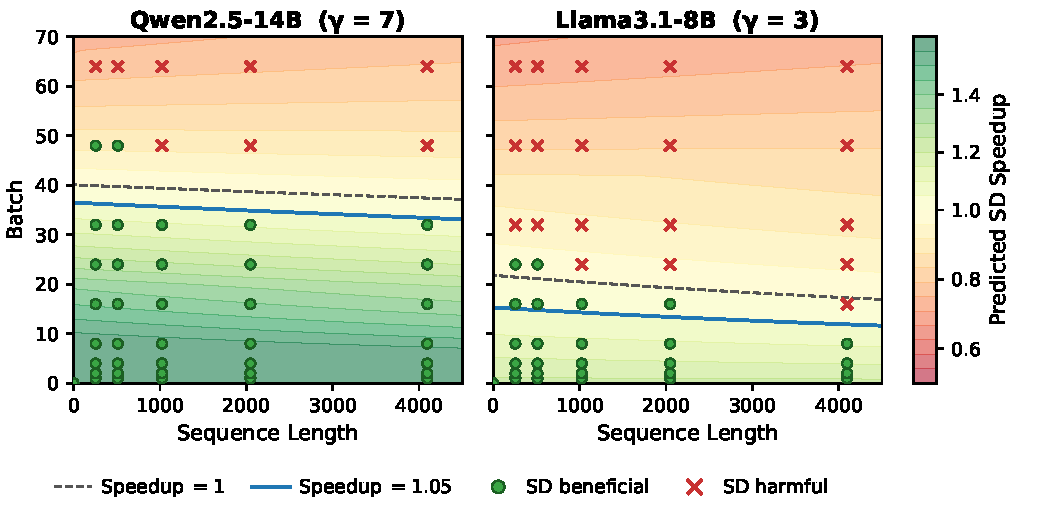
\includegraphics[width=\linewidth]{figures/main_sd_pair.pdf}
        \caption{
        \textbf{Validation of the roofline-based toggle boundary.}
        Colors show the predicted speedup over the batch-size and sequence-length plane, and markers indicate whether measured SD is beneficial or harmful at the corresponding coordinates.
        }
        \label{fig:toggle_boundary}
    \end{minipage}
    \hfill
    \begin{minipage}[t]{0.42\textwidth}
        \centering
        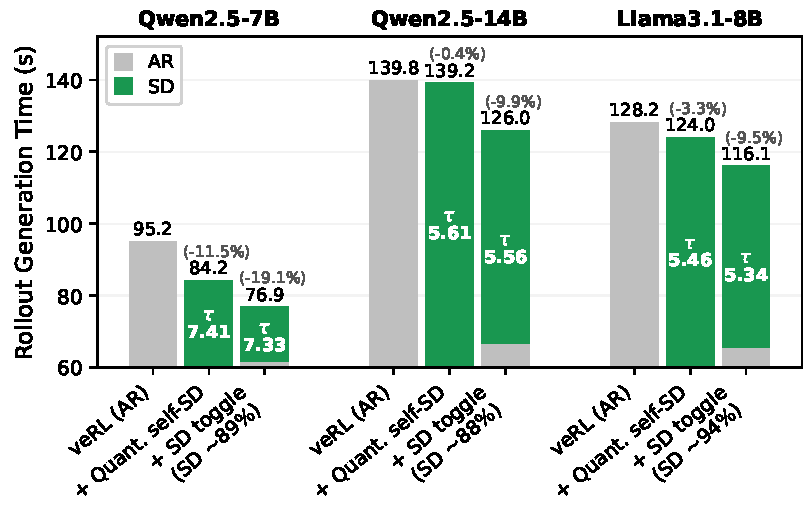
\includegraphics[width=\linewidth]{figures/main_toggle_vs_alwayson.pdf}
        \caption{
        \textbf{Effect of regime-aware SD toggling.}
        Average rollout time over the first 50 training steps, showing that toggling avoids harmful early-regime speculation across all evaluated models.
        }
        \label{fig:toggle_vs_alwayson}
    \end{minipage}

    \vspace{-0.5em}
\end{figure*}

\subsection{End-to-End RL Training Acceleration}
\label{subsec:eval-e2e-acceleration}

\textbf{End-to-end latency.}
\Cref{tab:e2e_speedup} shows that \methodtitle{} achieves the largest latency reduction among all methods for every evaluated model.
The per-step quantization overhead is modest (1.3--2.6\,s) relative to the rollout-time savings: \methodtitle{} reduces rollout-generation latency by up to \speeduprollout{}, yielding an end-to-end training-step latency reduction of up to \speedupete{} after accounting for all RL operations.
The \history{} baseline has the lowest preparation overhead from history lookup (1.1\,s), but does not reduce rollout-generation latency.
Even after rollout history becomes available, it reuses only 4.4--50.2\% of response tokens while adding 10.7--19.5\,s of verification overhead (\cref{tab:history_based_slow}).
Intuitively, prefix reuse acts like a large draft-and-verify block over the full candidate sequence, and even the highest reuse rate (50.2\%) is insufficient to amortize the added verification cost in our setting.
The \learned{} baseline shows model-dependent, limited gains because its auxiliary drafter does not consistently provide sufficient block efficiency to offset SD overheads (\cref{subsec:further-analysis}).
For example, it reduces Qwen2.5-14B step latency by 3.3\% but increases Llama3.1-8B step latency by 25.6\%.
Finally, \alwayssd{} reduces step latency on Qwen2.5-7B and Llama3.1-8B, but the Qwen2.5-14B slowdown shows that the quantized self-drafter alone is not sufficient for robust speedups.
We provide detailed analyses of slowdowns in the \history{} and \learned{} baselines in~\cref{app:why-history-slow,app:why-learned-auxiliary-challenging}.

\textbf{Acceptance rate and block efficiency.}
\Cref{tab:e2e_speedup} shows that \methodtitle{} attains consistently high $\alpha$ (95.8--98.2\%) together with large $\mal$.
\Alwayssd{} also maintains high $\alpha$ across models, indicating strong alignment between the target model and the quantized self-drafter.
\methodtitle{} preserves this high $\alpha$ while using larger $\bar{\gamma}$, indicating that adaptive $\gamma$ control can exploit training-time improvements in acceptance as it increases the draft budget.
By contrast, the \learned{} baseline remains limited to much lower $\alpha$ (54.3--60.3\%) even with shorter $\bar{\gamma}$, reflecting limited auxiliary-drafter effectiveness in long, high-temperature RL rollouts (\cref{subsec:further-analysis}).


\textbf{Training dynamics and quality preservation.}
\methodtitle{} accelerates training while preserving training dynamics.
\Cref{fig:adaptive_gamma_reward} shows that \methodtitle{} closely tracks the \nosd{} reward trajectory on Qwen2.5-7B.
This aligns with the lossless nature of SD, which preserves the target distribution~\citep{leviathan2023fast,chen2023accelerating} and is especially important in RL where rollout-distribution shifts can affect training stability~\citep{yu2025dapo,fu2025areal}.
Full reward and validation-accuracy trajectories across all evaluated models are provided in~\cref{app:quality-preservation}.

\begin{figure}[t]
    \centering

    \begin{subfigure}[t]{0.32\linewidth}
        \centering
        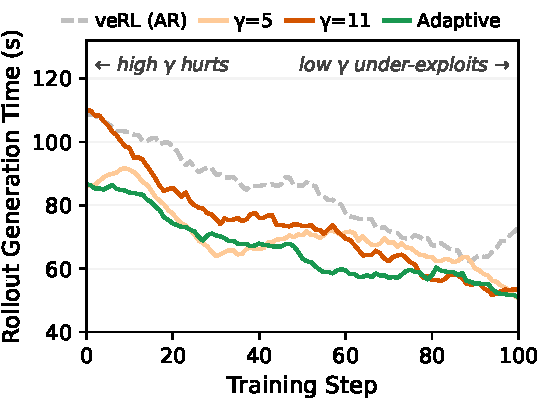
\includegraphics[width=\linewidth]{figures/main_adaptive_gen_time.pdf}
        \caption{Rollout generation time}
        \label{fig:adaptive_gamma_gen_time}
    \end{subfigure}
    \hfill
    \begin{subfigure}[t]{0.32\linewidth}
        \centering
        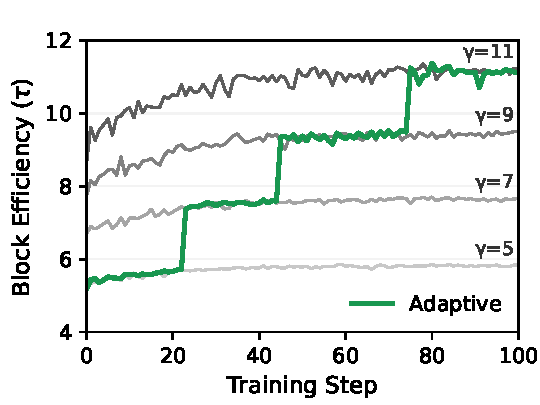
\includegraphics[width=\linewidth]{figures/main_adaptive_gamma.pdf}
        \caption{Block efficiency}
        \label{fig:adaptive_gamma_mal}
    \end{subfigure}
    \hfill
    \begin{subfigure}[t]{0.32\linewidth}
        \centering
        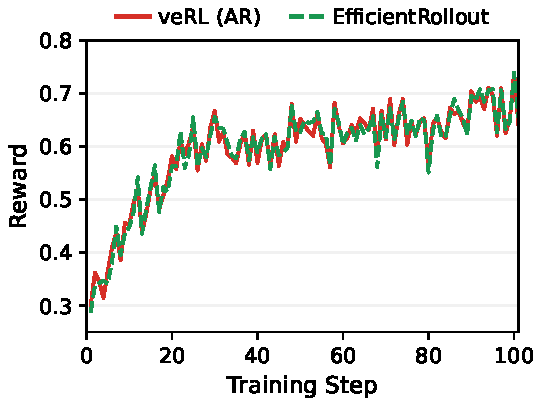
\includegraphics[width=\linewidth]{figures/appendix_fidelity_reward_qwen7b.pdf}
        \caption{Training reward}
        \label{fig:adaptive_gamma_reward}
    \end{subfigure}

    \caption{
    \textbf{Adaptive draft-length policy and training dynamics on Qwen2.5-7B.}
    (a) Adaptive $\gamma$ reduces rollout-generation time by avoiding overly large drafts early and exploiting longer drafts later.
    (b) The controller raises $\gamma$ as block efficiency $\tau$ improves during training.
    (c) \methodtitle{} follows the \nosd{} reward trajectory, indicating preserved training dynamics.
    }
    \label{fig:adaptive_gamma}
\end{figure}

\begin{wrapfigure}{r}{0.4\linewidth}
    \vspace{-13mm}
    \centering
    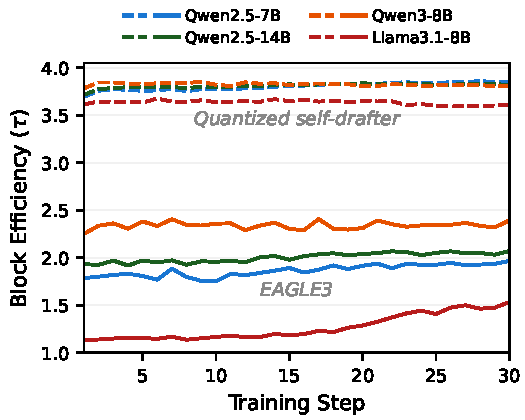
\includegraphics[width=0.97\linewidth]{figures/main_mal_combined.pdf}
    \vspace{-1mm}
    \caption{
    \textbf{Block efficiency across pretrained auxiliary drafters.}
    On DAPO-Math-17K, the evaluated pretrained auxiliary drafters achieve lower block efficiency than quantized self-drafters.
    }
    \label{fig:learned_auxiliary_mal_difficulty}
    \vspace{-4mm}
\end{wrapfigure}

\subsection{Further Analysis of Rollout Acceleration}
\label{subsec:further-analysis}

\textbf{Regime-aware SD toggle policy.}
High $\mal$ alone is insufficient for realized speedup, and SD must be activated only in system-beneficial regimes via the toggle policy $\SDToggle$.
\Cref{fig:toggle_boundary} validates the calibrated roofline boundary of $\SDToggle$ by showing that the predicted speedup correctly separates SD-beneficial and SD-harmful coordinates in the $(B,S)$ plane.
\Cref{fig:toggle_vs_alwayson} isolates the effect of $\SDToggle$ by comparing rollout latency with the same quantized self-drafter when SD is always enabled versus enabled according to $\SDToggle$.
By disabling SD during only the early 6--11\% of decoding steps, the $\SDToggle$ policy yields consistently larger rollout-generation latency reductions relative to AR than always-on SD, despite slightly lower $\mal$.
These gains therefore cannot be attributed to better draft quality; they come from avoiding verification in the initial large-batch regime, where $\VerifyTime/\TargetTime$ is high.
Full validation results for $\SDToggle$ are provided in~\cref{app:toggle_validation}.


\textbf{Adaptive draft-length policy.}
The adaptive $\DraftLength$ policy effectively tracks the latency-reducing $\DraftLength$ as the evolving target policy shifts over training.
We isolate this effect by replacing only the adaptive $\DraftLength$ policy in \methodtitle{} with fixed-$\DraftLength$ variants throughout training.
As shown in~\cref{fig:adaptive_gamma_gen_time}, the adaptive $\DraftLength$ policy achieves an overall 19.6\% reduction in rollout-generation latency, compared with 13.5\% and 11.8\% for fixed $\DraftLength{}=\gamma_{\mathrm{low}}=5$ and $\DraftLength{}=\gamma_{\mathrm{high}}=11$, respectively.
This improvement comes from leveraging larger latency reductions at different stages of training, as smaller and larger $\DraftLength$ values are more effective early and later in training, respectively.
Rather than selecting a single fixed $\DraftLength{}$ through post-hoc sweeps, the adaptive $\DraftLength$ policy moves within the pre-specified $\Gamma$ using observed $\mal$ feedback.

\textbf{Learned auxiliary drafting in RL workloads.}
The lower $\mal$ and $\alpha$ of \learned{} in~\cref{tab:e2e_speedup} reflect the practical difficulty of obtaining an auxiliary drafter aligned with long, high-temperature RL rollouts.
Under the prior RL-SD setup of \citet{iso2026accelerating}, we further evaluate auxiliary drafters on DAPO-Math-17K~\citep{yu2025dapo}, the rollout workload used in that setup.
As shown in~\cref{fig:learned_auxiliary_mal_difficulty}, the evaluated auxiliary drafters~\citep{redhatai2025llama31eagle3,redhatai2025qwen3eagle3thinking} achieve only $\mal=1.2$--$2.4$ over the first 30 steps, whereas the quantized self-drafter consistently reaches $\mal=3.6$--$3.9$ under the same setting.
These results suggest that directly reusing public checkpoints or drafters pretrained with fixed-target LLM-serving recipes~\citep{li2025eagle,zhang2025fastgrpo} is insufficient to reliably obtain high $\mal$ in RL rollouts.
Realizing effective speedups with \learned{} may require a more specialized auxiliary-drafter training pipeline~\citep{zhou2024distillspec, iso2026accelerating}, such as collecting in-distribution rollouts, training drafters on target-generated synthetic data, and possibly using more aggressive online adaptation.
Detailed evaluation settings and analyses with additional auxiliary-drafter checkpoints are presented in~\cref{app:workload-matched-auxiliary-drafters}.
